The Biot-Savard law, discovered in 1920 by French physicists Jean-Baptiste Biot and Felix Savard, is the fundamental law for understanding magnetism. The law is expressed as follows:

\begin{equation}
    \vec{B}=\frac{\mu_0}{4\pi}\frac{q\vec{v}\times\hat{r}}{r^2}
    \label{eq: Biot-Savard law}
\end{equation}

Where $\mu_o$ is the permeability constant \SI{4\pi e-7}{\tesla\metre\per\ampere}, $\vec{B}$ the magnetic field generated by some particle of charge $q$, $\vec{v}$ the particle's velocity, and $\hat{r}$ and $r$ are respectively a unit vector pointing from the particle to the point where the field is being calculated and the distance between said points. However, this law only applies to point charges. As such, we must adapt it to work with current segments. By definition, current is the rate of change of charge over time, that is 

\begin{equation}
    I\equiv\frac{\text{d} Q}{\text{d}t}
    \label{eq: Current definition}
\end{equation}

Furthermore, in any given section of wire $\Delta\vec{s}$, the velocity of the moving charges is parallel to the segment itself. Therefore, we can rewrite the Biot-Savard law for current segments as,

\begin{equation}
    \vec{B}_{\substack{\text{current}\\ \text{segment}}}=\frac{\mu_0}{4\pi}\frac{I\Delta\vec{s}\times\hat{r}}{r^2}
    \label{eq: Current Biot-Savard}
\end{equation}

Now, we can use this equation to find the magnetic field of a coil. Figure \ref{fig:Situation representation} shows a simple representation of our situation. 

\begin{figure}
    \centering
    \usetikzlibrary {3d}
        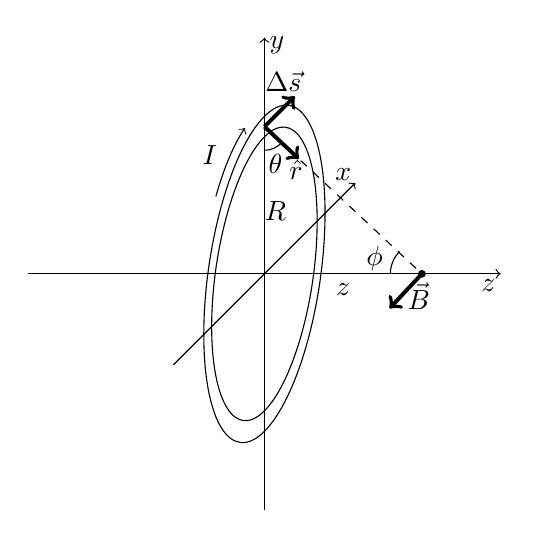
\begin{tikzpicture}[scale=2]
            \begin{scope}[canvas is zy plane at x=0]
              \draw (0,0) circle (1cm);
              \draw (0,0) circle (0.87cm);
              \draw[->] (1.5,0) -- (-1.5,0);
              \draw[line width = 0.5mm, ->] (0,0.935cm) -- (-0.5,0.935cm);
              \draw[->] (0.8,0.8) arc (45:80:0.9);
              \draw node at (0.9,1.1) {$I$};
              \draw node at (-1.3,0.13) {$x$};
            \end{scope}
        
           \begin{scope}[canvas is zx plane at y=0]
              \draw[->] (0,-1.5) -- (0,1.5);
              \draw node at (0.2,1.5) {$z$};
            \end{scope}
        
            \begin{scope}[canvas is xy plane at z=0]
              \draw[->] (0,-1.5) -- (0,1.5);
              \draw[dashed] (0,0.935cm) -- (1,0);
              \draw[line width = 0.5mm, ->] (0,0.935cm) -- (0.219,0.73);
              \draw node at (1,0) [circle, fill = black, scale = 0.3]{};
              \draw[line width = 0.5mm, ->] (1,0) -- (0.795,-0.219);
              \draw (0,0.785cm) arc (270:317:0.15cm);
              \draw (0.8,0) arc (180:135:0.2cm);
              \draw node at (0.12,1.22) {$\Delta\vec{s}$};
              \draw node at (0.2,0.66) {$\hat{r}$};
              \draw node at (0.07,0.4) {$R$};
              \draw node at (0.07,0.7) {$\theta$};
              \draw node at (0.7,0.1) {$\phi$};
              \draw node at (0.5,-0.1) {$z$};
              \draw node at (0.98,-0.14) {$\vec{B}$};
              \draw node at (0.08,1.45) {$y$};
            \end{scope}
 \end{tikzpicture}
    \caption{Representation of a current carrying coil segment and its magnetic field at a point on the z-axis. Where z is the distance from the center of the coil to the point on the z-axis.}
    \label{fig:Situation representation}
\end{figure}

From the Biot-Savard law we know that $\vec{B}$ must be perpendicular to $\Delta\vec{s}$ and $\hat{r}$, as shown in the figure. If we pair our segment with one \SI{180}{\degree} away, we can see that the $x$ and $y$ components would cancel, leaving only the $z$ component. This is true for all segments; therefore we need only add the $z$ components of each segment. Here, this component is given by $B_z=B\cos(90\degree-\phi)$, which is simply $B\cos\theta$ since $\theta=90\degree-\phi$. Finally, since $\cos\theta=R/r$, we write the Biot-Savard law as follows,

\begin{equation}
    B_z=\frac{\mu_0}{4\pi}\frac{I\Delta\vec{s}\times\hat{r}}{r^2}\cos\theta=\frac{\mu_0IR}{4\pi r^3}\Delta{s}
    \label{eq: Loop segment incomplete}
\end{equation}

Note that $\Delta\vec{s}\times\hat{r}=\Delta s(1)\sin(90\degree)=\Delta s$. Next, we observe that by the Pythagorean theorem $r=(z^2+R^2)^{1/2}$. Thus we rewrite equation \eqref{eq: Loop segment incomplete} as,

\begin{equation}
    B_z=\frac{\mu_0IR}{4\pi(z^2+R^2)^{3/2}}\Delta s
    \label{eq: Loop segment comlpete}
\end{equation}

Now, the last step is to add all the loop segments together:

\begin{equation*}
    B_{\text{net}}=\sum_i(B_i)_z=\frac{\mu_0IR}{4\pi(z^2+R^2)^{3/2}}\sum_i\Delta s
\end{equation*}

Here, we factored all constant terms leaving only $\Delta s$ inside the sum, which is simply the length of the coil, $2\pi R$. Replacing this into our equation, we reach our final result:

\begin{equation}
    {B}_{\text{net}}=\frac{\mu_0IR}{4\pi(z^2+R^2)^{3/2}}\times2\pi R=\frac{\mu_0IR^2}{2(z^2+R^2)^{3/2}}
    \label{eq: Loop final equation}
\end{equation}

Finally, because magnetic fields follow superposition, we multiply this equation by the number of loops to find the equation for a coil with $N$ loops:

\begin{equation}
    {B}_{\substack{\text{coil} \\ \text{on-axis}}}=N\frac{\mu_0IR^2}{2(z^2+R^2)^{3/2}}
\end{equation}